\documentclass{article}

\usepackage[dvipsnames]{xcolor}
\usepackage{ctex}
\usepackage{graphicx}
\usepackage[unicode]{hyperref}
\usepackage{cite}
\usepackage{indentfirst}
\usepackage{listings}
\usepackage{geometry}
\usepackage{amsmath}

\geometry{a4paper, left=2cm, right=2cm, top=1cm, bottom=1.5cm}

% \lstset{
%   language=C++,
%   basicstyle=\fontsize{8}{5}\ttfamily, % 设置代码字体大小为 12pt
%   breaklines=true, % 自动换行
%   numbers=left,
%   showstringspaces = false
% }

%%%%%% 设置字号 %%%%%% 
\newcommand{\chuhao}{\fontsize{nn42pt}{\baselineskip}\selectfont}
\newcommand{\xiaochuhao}{\fontsize{36pt}{\baselineskip}\selectfont}
\newcommand{\yihao}{\fontsize{28pt}{\baselineskip}\selectfont}
\newcommand{\erhao}{\fontsize{21pt}{\baselineskip}\selectfont}
\newcommand{\xiaoerhao}{\fontsize{18pt}{\baselineskip}\selectfont}
\newcommand{\sanhao}{\fontsize{15.75pt}{\baselineskip}\selectfont}
\newcommand{\sihao}{\fontsize{14pt}{\baselineskip}\selectfont}
\newcommand{\xiaosihao}{\fontsize{12pt}{\baselineskip}\selectfont}
\newcommand{\wuhao}{\fontsize{10.5pt}{\baselineskip}\selectfont}
\newcommand{\xiaowuhao}{\fontsize{9pt}{\baselineskip}\selectfont}
\newcommand{\liuhao}{\fontsize{7.875pt}{\baselineskip}\selectfont}
\newcommand{\qihao}{\fontsize{5.25pt}{\baselineskip}\selectfont}

% %%%% 设置 section 属性 %%%%
% \makeatletter
% \renewcommand\section{\@startsection{section}{1}{\z@}%
% {-1.5ex \@plus -.5ex \@minus -.2ex}%
% {.5ex \@plus .1ex}%
% {\normalfont\sihao\CJKfamily{hei}}}
% \makeatother

 %%%% 设置 subsection 属性 %%%%
% \makeatletter
% \renewcommand\subsection{\@startsection{subsection}{1}{\z@}%
% % {-1.25ex \@plus -.5ex \@minus -.2ex}%
% % {-1ex \@plus -.5ex \@minus -.2ex}%
% {-1ex \@plus -.3ex \@minus -.1ex}%
% {.4ex \@plus .1ex}%
% {\normalfont\xiaosihao\CJKfamily{hei}}}
% \makeatother

% %%%% 设置 subsubsection 属性 %%%%
% \makeatletter
% \renewcommand\subsubsection{\@startsection{subsubsection}{1}{\z@}%
% {-1ex \@plus -.5ex \@minus -.2ex}%
% {.3ex \@plus .1ex}%
% {\normalfont\xiaosihao\CJKfamily{hei}}}
% \makeatother

%%%% 段落首行缩进两个字 %%%%
\makeatletter
\let\@afterindentfalse\@afterindenttrue
\@afterindenttrue
\makeatother
% \setlength{\parindent}{2em}  %中文缩进两个汉字位

%%%% 下面的命令重定义页面边距,使其符合中文刊物习惯 %%%%
% \addtolength{\topmargin}{-54pt}
% \setlength{\oddsidemargin}{0.63cm}  % 3.17cm - 1 inch
% \setlength{\evensidemargin}{\oddsidemargin}
% \setlength{\textwidth}{14.66cm}
% \setlength{\textheight}{24.00cm}    % 24.62

%%%% 下面的命令设置行间距与段落间距 %%%%
\linespread{1.0}
% \setlength{\parskip}{1ex}
\setlength{\parskip}{0.5\baselineskip}

% 在导言区进行样式设置
\lstset{
    language=C++, % 设置语言
 	basicstyle=\ttfamily, % 设置字体族
 	breaklines=true, % 自动换行
 	keywordstyle=\bfseries\color{NavyBlue}, % 设置关键字为粗体,颜色为 NavyBlue
 	morekeywords={PressureSensor, Button, Oled}, % 设置更多的关键字,用逗号分隔
 	emph={self}, % 指定强调词,如果有多个,用逗号隔开
    emphstyle=\bfseries\color{Rhodamine}, % 强调词样式设置
    commentstyle=\itshape\color{black!50!white}, % 设置注释样式,斜体,浅灰色
    stringstyle=\bfseries\color{PineGreen!90!black}, % 设置字符串样式
    columns=flexible,
    numbers=left, % 显示行号在左边
    numbersep=2em, % 设置行号的具体位置
    numberstyle=\footnotesize, % 缩小行号
    % frame=single, % 边框
	tabsize = 4,  %行缩进
    framesep=1em % 设置代码与边框的距离
}

%%%% 正文开始 %%%%
\begin{document}	
		%%%% 定理类环境的定义 %%%%
\newtheorem{example}{例}             % 整体编号
\newtheorem{algorithm}{算法}
\newtheorem{theorem}{定理}[section]  % 按 section 编号
\newtheorem{definition}{定义}
\newtheorem{axiom}{公理}
\newtheorem{property}{性质}
\newtheorem{proposition}{命题}
\newtheorem{lemma}{引理}
\newtheorem{corollary}{推论}
\newtheorem{remark}{注解}
\newtheorem{condition}{条件}
\newtheorem{conclusion}{结论}
\newtheorem{assumption}{假设}

		%%%% 重定义 %%%%
\renewcommand{\contentsname}{目录}  % 将Contents改为目录
\renewcommand{\abstractname}{摘要}  % 将Abstract改为摘要
\renewcommand{\refname}{参考文献}   % 将References改为参考文献
\renewcommand{\indexname}{索引}
\renewcommand{\figurename}{图}
\renewcommand{\tablename}{表}
\renewcommand{\appendixname}{附录}
\renewcommand{\algorithm}{算法}	

		%%% 定义标题格式,包括title,author,affiliation,email等 %%%%
\title{智能仓储系统的开发研究}
% \author{XXX\footnote{电子邮件: XXXXXXXXXXXX@zjut.edu.cn 学号: XXXXXXXXXXXX}\\[2ex]
% \xiaosihao 浙江工业大学\\[2ex]}
\author{\xiaosihao 先进计算与机器人研究所}
%\date{}
		
		%%%% 以下部分是正文 %%%%  
\maketitle
		
\tableofcontents
\newpage

\section{第七章: 部署}
这一章主要介绍实际如何部署好一个货架。一个完整的货架包含: 一个触摸屏, 多个电子秤还有整个架子。软件上需要给所有电子秤烧录好代码, 触摸屏的UI界面设计好; 
硬件上要连好Arduino和压力传感器, 读卡器等元器件的连线, 以及整个货架的IIC通信线路。上述过程分为四步来完成:
\begin{itemize}
  \item 第一步: 秤的组装;
  \item 第二步: 上传程序;
  \item 第三步: 货架布线;
  \item 第四步: 触摸屏显示;
\end{itemize}

\subsection{秤的组装}
压力测量模块连接, 详见第一章:
\begin{figure}[h]
	\centering
	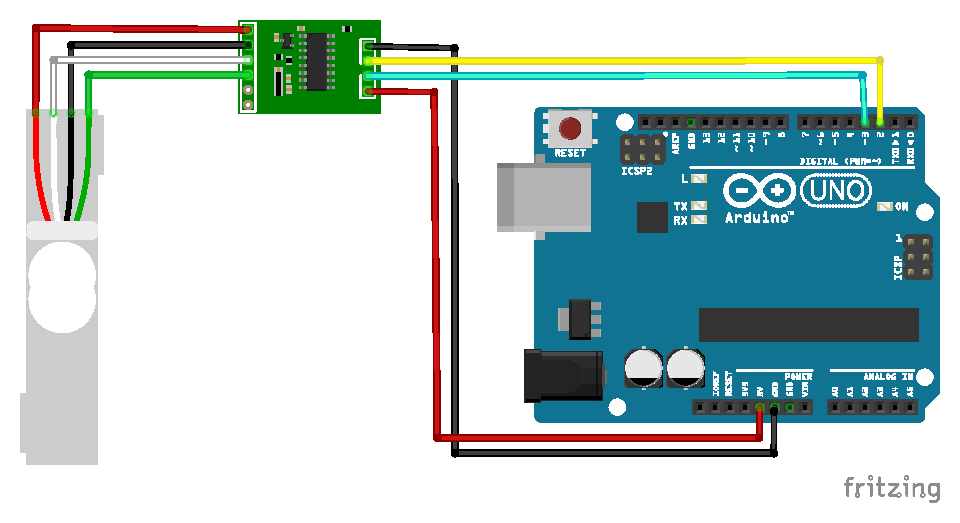
\includegraphics[width=\linewidth]{../../1_Chapter1_RAW/Picture/PressureSensor.pdf}
	\caption{压力测量模块流程}
	\label{fig:压力测量模块流程图}
	\hfill
\end{figure}
		
两种读卡器连接, 详见第五章第六章:
\begin{figure}[h]
	\centering
	\begin{minipage}{.45\textwidth}
		\centering
		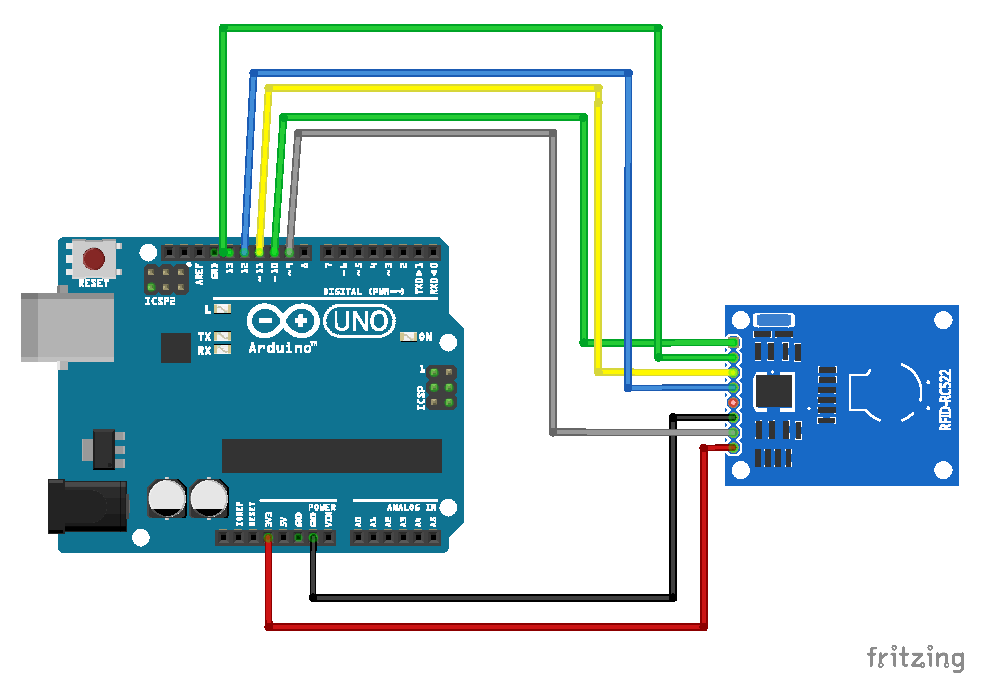
\includegraphics[width=\linewidth]{../../5_Chapter5_RC522/Picture/RFID_RC522.pdf}
		\caption{RC522硬件连接}
		\label{fig:RC522硬件连接}
	\end{minipage}%
	\hfill
  \begin{minipage}{.45\textwidth}
		\centering
		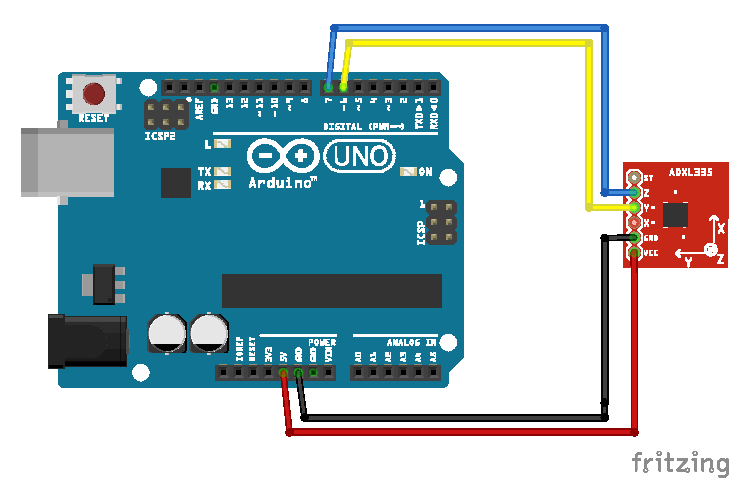
\includegraphics[width=\linewidth]{../../6_Chapter6_UHF_R505/Picture/R505.pdf}
		\caption{R505 与 arduino的实物连接图}
		\label{fig:R505 与 arduino的实物连接图}
	\end{minipage}
\end{figure}

\subsection{上传程序}
这里我们选择的是TCA9548A的布线方式, arduino分为多个主机一个从机, 

\noindent 主机:
如果是采取近的读卡器读取物品种类及单个物体质量信息, 就烧录下面的程序:
\begin{lstlisting}
  #include "master.h"
  #include "transform.h"
  #include "Surface.h"
  #include "Calibrate.h"
  #include "Oled.h"
  #include "RC522.h"
  
  master m1;
  Surface YL_Surface;
  Calibrate YL_Calibrated;
  transform tf;
  Oled oled;
  RC522 rc522;
  
  long numbefore=0, numnow=1;
  char te[3];
  unsigned long Sweight;
  bool rflag=1;  //1 ---> read; 0 ---> write
  
  void setup() {
    Serial.begin(9600);
    m1.initialize(8);    //8needschanged
    YL_Calibrated.setpin_SCKDT(4, 5);
    YL_Calibrated.set_range(20);
    YL_Calibrated.kb_Initialize();
    oled.initialize();  
    rc522.initialize(9,10);
  }
  
  void loop() {
    switch(rflag){
      case 0: 
        while(1) {
          bool state = rc522.write();
          if(state==1)
            break;
        }   
        rflag=1;
        break;
      case 1:
        while(1) {
          bool state = rc522.read();
          if(state==1)
            break;
        }
        break;
    }
    for (int i=0; i<sizeof(rc522.Type_Name);i++) te[i]=rc522.Type_Name[i];
    Sweight=rc522.Single_Weight;
  
    numbefore = numnow;
    unsigned long CalibratedWeight = YL_Calibrated.Output_CalibratedWeight(YL_Surface.Get_Surface());
    numnow = ceil(CalibratedWeight/Sweight);
  
    bool flag= (numbefore==numnow?0:1);
    if(flag){
    tf.initialize(te, m1.address, numnow, CalibratedWeight);
    tf.pack();
    digitalWrite(3,HIGH);
    m1.send(9, tf.Transmission_Information);
    Serial.println(tf.Transmission_Information);
    oled.showIIC(te, numnow);
    digitalWrite(3,LOW);
    }
  
    delay(3000);
  }  
\end{lstlisting}

如果是采取远的读卡器读取物品种类及单个物体质量信息, 就烧录下面的程序:
\begin{lstlisting}
  #include "master.h"
  #include "transform.h"
  #include "Surface.h"
  #include "Calibrate.h"
  #include "Oled.h"
  #include "RC522.h"
  #include "RC505.h"
  
  master m1;
  Surface YL_Surface;
  Calibrate YL_Calibrated;
  transform tf;
  Oled oled;
  RC522 rc522;
  RC505 rc505;
  
  long numbefore=0, numnow=1;
  char te[3];
  unsigned long Sweight;
  char MessageNow[arrayMax];
  bool flag=0; //1--->write; 0--->read
  
  void setup() {
    //设置串口波特率38400
    Serial.begin(38400);
    m1.initialize(8);    //8needschanged
    YL_Calibrated.setpin_SCKDT(4, 5);
    YL_Calibrated.set_range(20);
    YL_Calibrated.kb_Initialize();
    oled.initialize();  
    rc522.initialize(9,10);
  }
  
  
  void loop() { 
    switch(flag){
      case 0: 
        // while(1) {
        //   bool state = rc505.write();
        //   if(state==1)
        //     break;
        // }   
        rflag=1;
        // break;
      case 1:
        while(1) {
          bool state = rc505.read(MessageNow);
          if(state==1)
            break;
        }
        break;
    }  
    for (int i=0; i<sizeof(rc505.Type_Name);i++) te[i]=rc505.Type_Name[i];
    Sweight=rc505.Single_Weight;
  
    numbefore = numnow;
    unsigned long CalibratedWeight = YL_Calibrated.Output_CalibratedWeight(YL_Surface.Get_Surface());
    numnow = ceil(CalibratedWeight/Sweight);
  
    bool flag= (numbefore==numnow?0:1);
    if(flag){
    tf.initialize(te, m1.address, numnow, CalibratedWeight);
    tf.pack();
    digitalWrite(3,HIGH);
    m1.send(9, tf.Transmission_Information);
    Serial.println(tf.Transmission_Information);
    oled.showIIC(te, numnow);
    digitalWrite(3,LOW);
    }
  
    delay(3000); 
  }
\end{lstlisting}

\noindent 从机(也就是与TCA9548A相连的arduino板上的主程序如下):
\begin{lstlisting}
#include "Oled.h"
#include "slave.h"
#include "transform.h"

String slave::comdata="";

Oled oled;
slave s;
transform tf;

void setup() {
  Serial.begin(9600);
  s.initialize(8);
  oled.initialize();
  pinMode(7,INPUT);
  digitalWrite(7, LOW);
}

void loop() {
  tf.unpack(s.comdata);
  oled.showIIC(tf.Type_Name, tf.Number, tf.DEVICE_ADDRESS);
  delay(1000);
}
\end{lstlisting}

\newpage
\subsection{货架布线}
IIC通信及OLED屏显示连线, 详见第三章第四章:
\begin{figure}[h]
  \centering
  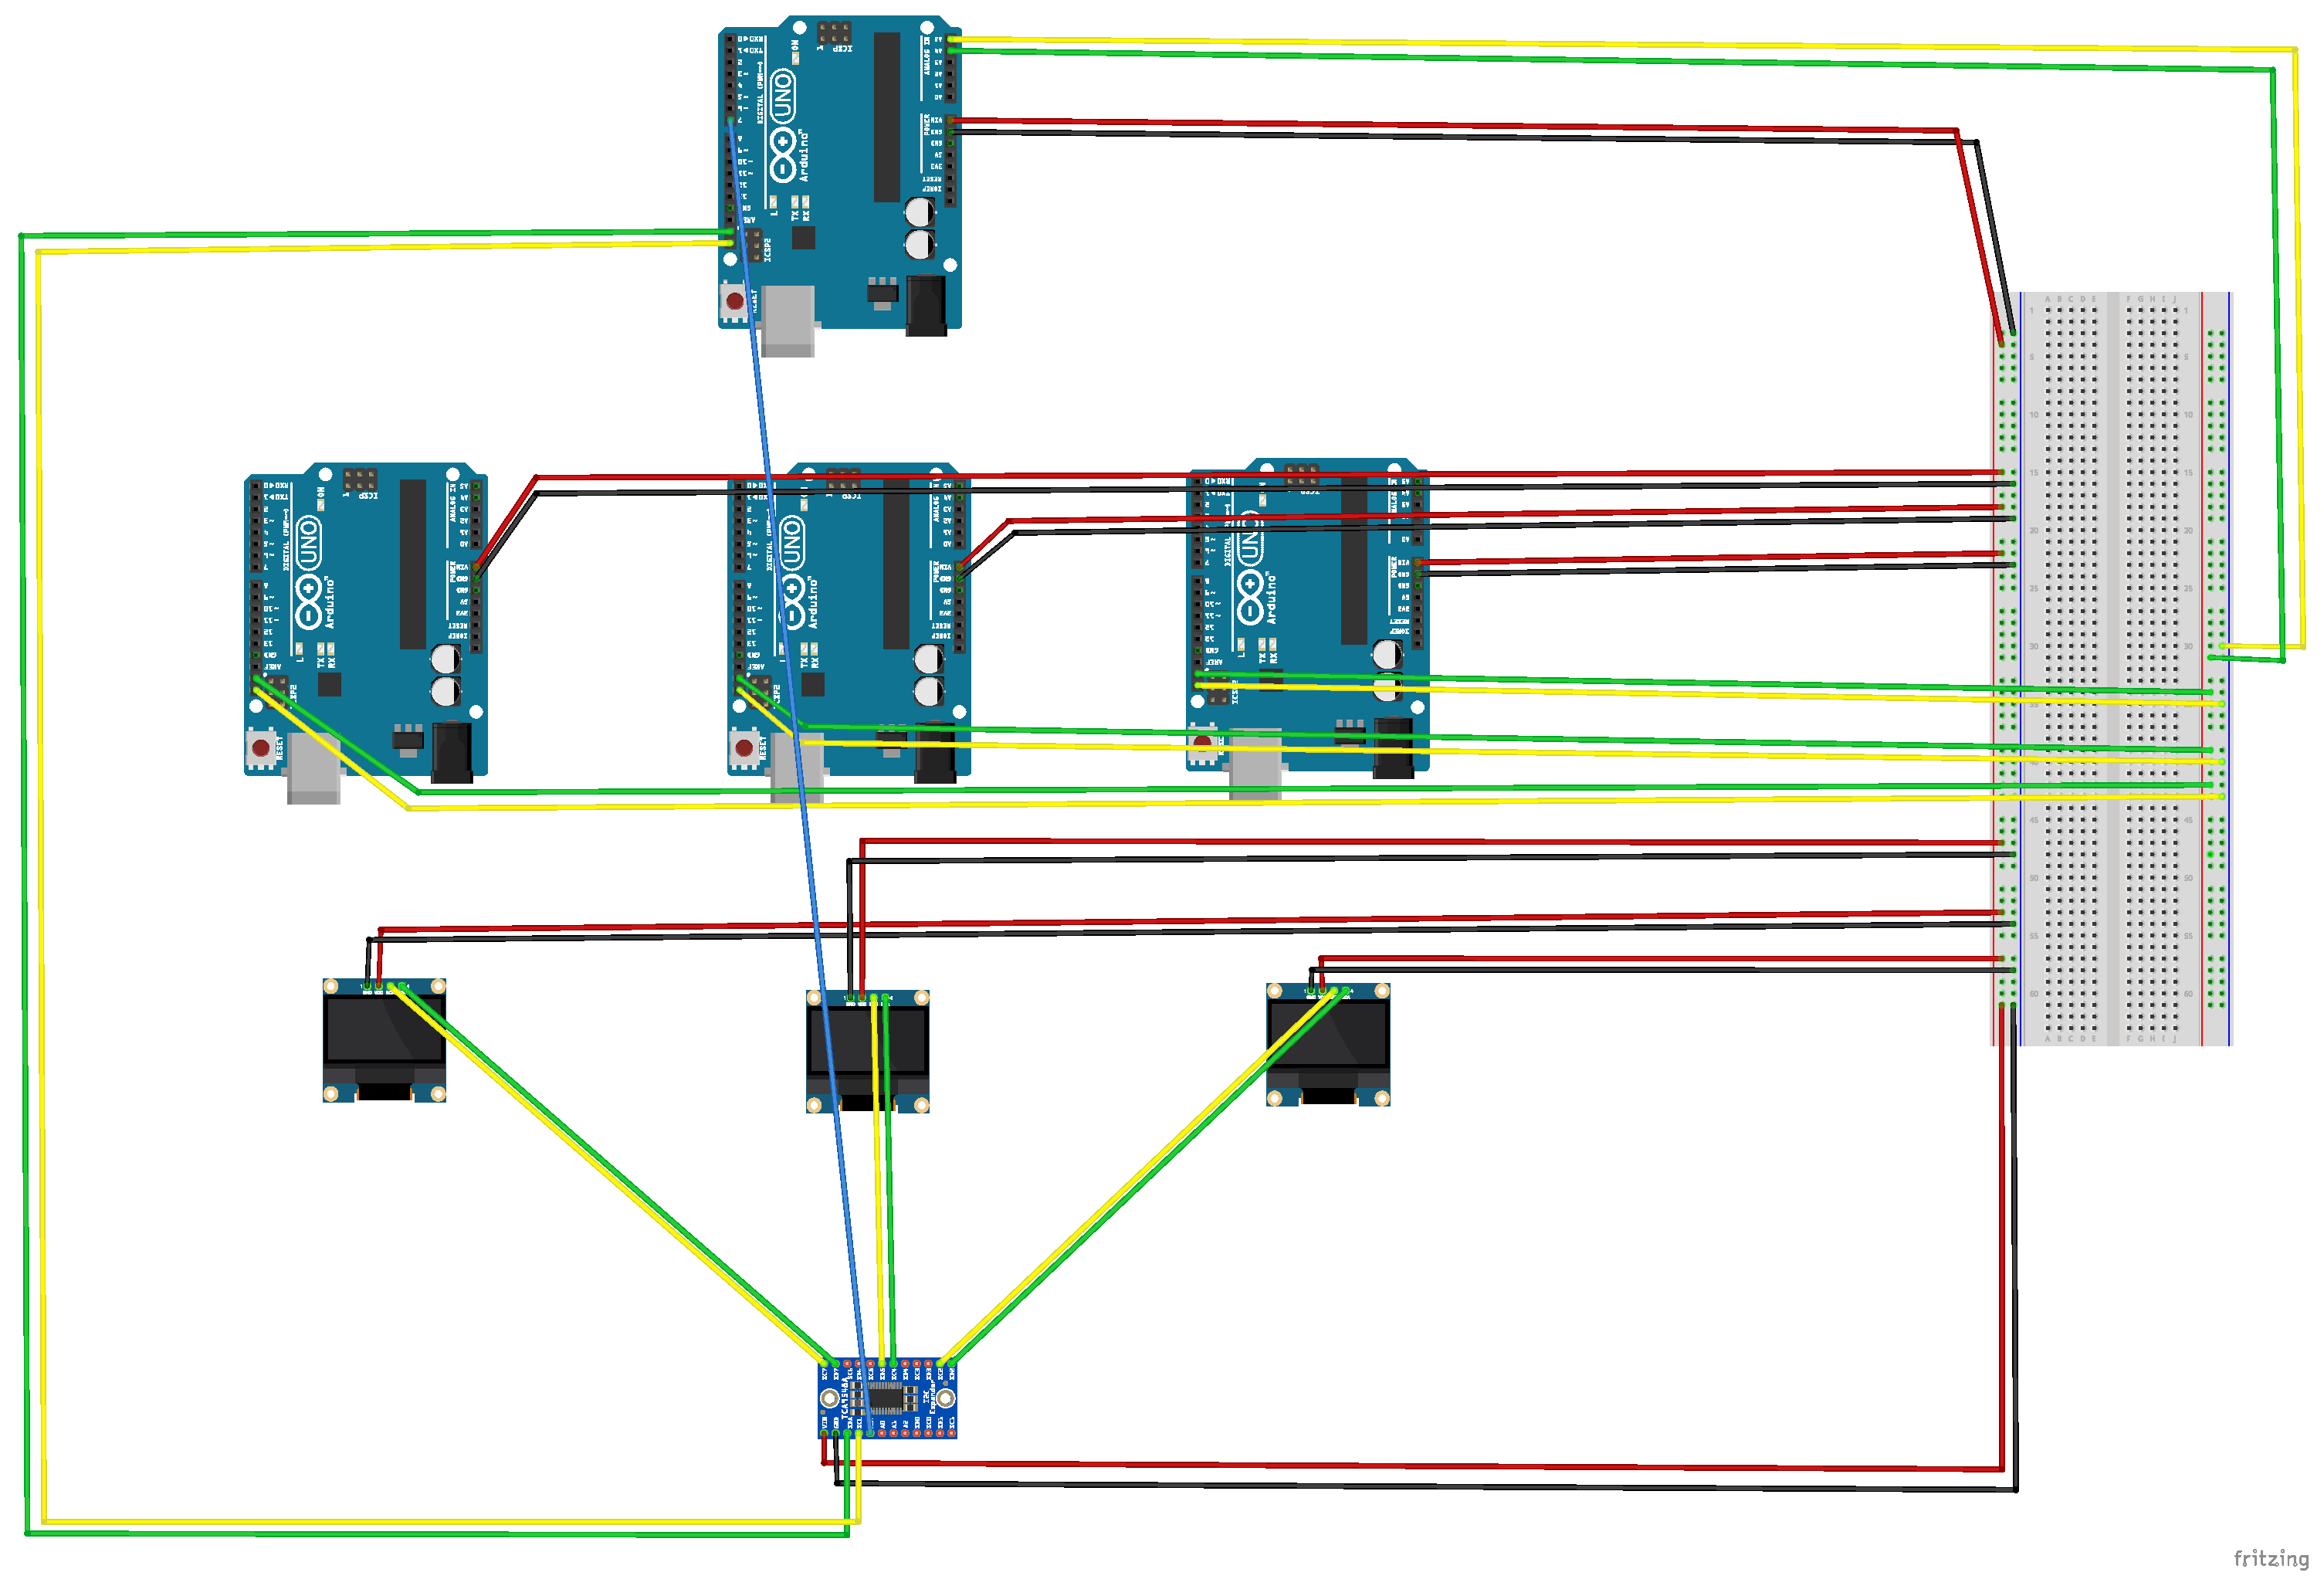
\includegraphics[width=0.8\textwidth]{../../4_Chapter4_COMMUNICATION/Picture/一层货架示意图.pdf}
  \caption{一层货架示意图}
  \label{fig:一层货架示意图}
\end{figure}

对于第二层甚至更多层的话, 就要考虑总的电子秤数量是否超过8, 超过了的话则需要更多从机和TCA9548A模块。

\subsection{触摸屏显示}
上传下面的python代码到树莓派上运行, 树莓派就可以接收到从机发来的信号, 从而在屏幕上显示对应电子秤的重量变化。

\begin{lstlisting}
import sys
from PyQt5.QtWidgets import QApplication, QWidget, QVBoxLayout, QHBoxLayout, QGridLayout, QLabel, QMainWindow
from PyQt5.QtGui import QPixmap
from PyQt5.QtCore import Qt, QTimer, QIODevice, QByteArray
from PyQt5.QtSerialPort import QSerialPort, QSerialPortInfo
from qt_material import apply_stylesheet
from PyQt5.uic import loadUi


class MainWindow(QMainWindow):
    def __init__(self):
        super().__init__()
        loadUi("main_window1.ui", self)  # 加载UI文件
        # 设置窗口标题和大小
        self.setWindowTitle('货物管理')

        # 创建网格布局
        grid = QGridLayout(self)
        grid.setAlignment(Qt.AlignCenter)

        pixmap = QPixmap('jimu1.jpg')
        pixmap = pixmap.scaled(150, 130, Qt.KeepAspectRatio)
        self.label1.setPixmap(pixmap)
        self.label1.setFixedSize(pixmap.width(), pixmap.height())
        self.label1.setAlignment(Qt.AlignCenter)
        self.pushButton.clicked.connect(self.click_button)
        self.pushButton_2.clicked.connect(self.click_button2)

        # 应用Qt Material主题
        apply_stylesheet(self, theme='light_teal.xml')

        # 创建串口监视器
        self.serial = QSerialPort()
        self.serial.setPortName("COM3")  # 设置端口号
        self.serial.setBaudRate(QSerialPort.Baud9600)
        self.serial.readyRead.connect(self.handle_serial_data)
        self.serial.open(QIODevice.ReadWrite)

    def click_button(self):
        self.serial.close()

    def click_button2(self):
        self.serial = QSerialPort()
        self.serial.setPortName("COM8")  # 设置端口号
        self.serial.setBaudRate(QSerialPort.Baud9600)
        self.serial.readyRead.connect(self.handle_serial_data)
        self.serial.open(QIODevice.ReadWrite)

    def handle_serial_data(self):
        # 读取串口数据
        data = self.serial.readAll().data()
        data_str = str(data, encoding='utf-8')
        print(data)
        # 处理数据
        module_data = data_str.split(',')
        for i, module_str in enumerate(module_data):
            # 如果模块数据不为空,则更新数量和种类
            if module_str:
                try:
                    type_, num = module_str.split(':')
                    self.update_module_info(i, type_, num)
                except ValueError as e:
                    print(f"Error: {e}. Received data: {module_str}")

    def update_module_info(self, module_num, type_, num):
        # 获取模块信息字典
        module_info = {
            0: {'num': None, 'type': 'AA', 'image': 'jimu1.jpg'},
            1: {'num': None, 'type': 'B', 'image': 'picture2.jpg'},
            2: {'num': None, 'type': 'C', 'image': 'picture3.jpg'},
            3: {'num': None, 'type': 'D', 'image': 'picture4.jpg'},
            4: {'num': None, 'type': 'E', 'image': 'picture5.jpg'},
            5: {'num': None, 'type': 'F', 'image': 'picture6.jpg'},
            6: {'num': None, 'type': 'G', 'image': 'picture7.jpg'},
            7: {'num': None, 'type': 'H', 'image': 'picture8.jpg'},
            8: {'num': None, 'type': 'I', 'image': 'picture9.jpg'},
            9: {'num': None, 'type': 'J', 'image': 'picture10.jpg'},
            10: {'num': None, 'type': 'K', 'image': 'picture11.jpg'},
            11: {'num': None, 'type': 'L', 'image': 'picture12.jpg'}
        }

        # 更新模块信息字典中对应模块的数量和种类
        for i in range(12):
            if module_info[i]['type'] == type_:
                module_info[i]['num'] = num
                num_label = self.findChild(QLabel, f'label_num_{i}')
                type_label = self.findChild(QLabel, f'label_type_{i}')
                if num_label is None:
                    print(f"label_num_{module_num} not found!")
                    return

                num_label.setText(num)
                break


if __name__ == '__main__':
    app = QApplication(sys.argv)
    main_window = MainWindow()
    main_window.show()
    sys.exit(app.exec_())  
\end{lstlisting}

\end{document} 

